% ****** Start of file apssamp.tex ******
%
%   This file is part of the APS files in the REVTeX 4.1 distribution.
%   Version 4.1r of REVTeX, August 2010
%
%   Copyright (c) 2009, 2010 The American Physical Society.
%
%   See the REVTeX 4 README file for restrictions and more information.
%
% TeX'ing this file requires that you have AMS-LaTeX 2.0 installed
% as well as the rest of the prerequisites for REVTeX 4.1
%
% See the REVTeX 4 README file
% It also requires running BibTeX. The commands are as follows:
%
%  1)  latex apssamp.tex
%  2)  bibtex apssamp
%  3)  latex apssamp.tex
%  4)  latex apssamp.tex
%
\documentclass[%
 preprint,
%superscriptaddress,
%groupedaddress,
%unsortedaddress,
%runinaddress,
%frontmatterverbose, 
%preprint,
%showpacs,preprintnumbers,
%nofootinbib,
%nobibnotes,
%bibnotes,
 amsmath,amssymb,
 aps,
%pra,
%prb,
%rmp,
%prstab,
%prstper,
%floatfix,
]{revtex4-1}

\usepackage{graphicx}% Include figure files
\usepackage{dcolumn}% Align table columns on decimal point
\usepackage{bm}% bold math
%\usepackage{hyperref}% add hypertext capabilities
%\usepackage[mathlines]{lineno}% Enable numbering of text and display math
%\linenumbers\relax % Commence numbering lines

%\usepackage[showframe,%Uncomment any one of the following lines to test 
%%scale=0.7, marginratio={1:1, 2:3}, ignoreall,% default settings
%%text={7in,10in},centering,
%%margin=1.5in,
%%total={6.5in,8.75in}, top=1.2in, left=0.9in, includefoot,
%%height=10in,a5paper,hmargin={3cm,0.8in},
%]{geometry}

\usepackage{braket} % Allows for Dirac notation
\usepackage{subcaption}

\newcommand{\veff}{\hat{V}_{12,\text{eff}}}
\newcommand{\rhozero}{\rho_{\text{I}=0}}
\newcommand{\rhoone}{\rho_{\text{I}=1}}

\newcommand{\rhohat}[2]{\hat{\rho}_{\text{I}=#1}\left( #2 \right)}

\newcommand{\yukawa}[1]{\frac{e^{-m_\pi |#1|}}{4\pi |#1|}}
\newcommand{\yukawadimless}[1]{\frac{e^{-m_\pi #1}}{m_\pi #1}}
\newcommand{\yukawanoabs}[1]{\frac{e^{-m_\pi #1}}{4\pi #1}}

\newcommand{\rot}{\vec{r}_{12}}
\newcommand{\rotp}{\vec{r}_{12}\!\!\!'\,\,}

\newcommand{\rotpr}{r_{12}\!\!\!\!'\,\,\,}
\newcommand{\rotphat}{\hat{r}_{12}\!\!\!\!'\,\,\,}

\newcommand{\taudot}{\vec{\tau}_1\cdot\vec{\tau}_2}
\newcommand{\taucrossthree}{\left[\vec{\tau}_1\times\vec{\tau}_2\right]_3}
\newcommand{\tauplusthree}{\frac{\tau_1^3+\tau_2^3}{2}}
\newcommand{\tauminusthree}{\frac{\tau_1^3+\tau_2^3}{2}}

\newcommand{\sigmadot}{\vec{\sigma}_1\cdot\vec{\sigma}_2}
\newcommand{\sigmaplus}{\vec{\sigma}_1+\vec{\sigma}_2}
\newcommand{\sigmaminus}{\vec{\sigma}_1-\vec{\sigma}_2}
\newcommand{\sigmatwo}{[\vec{\sigma}_1\otimes\vec{\sigma}_2]_2}
\newcommand{\sigmaone}{[\vec{\sigma}_1\otimes\vec{\sigma}_2]_1}
\newcommand{\sigmacross}{\vec{\sigma}_1\times\vec{\sigma}_2}

\newcommand{\fracphantom}{\vphantom{\frac{1}{1}}}

\newcommand{\lvec}[1]{\reflectbox{\ensuremath{\vec{\reflectbox{\ensuremath{#1}}}}}}

%\newcommand{\w}[4]{w(#1,#2,#3;#4)}
\newcommand{\w}[4]{w_{#1,#2,#3}(#4)}

\begin{document}

\preprint{APS/123-QED}

\title{An Analytic Reduction of the Chiral Three-Nucleon Potential to an In-Medium Two-Nucleon Form}% Force line breaks with \\
%\thanks{A footnote to the article title}%

\author{Cory D. Schillaci}
\email{schillaci@berkeley.edu}
%\author{Mark C. Strother}
%\email{mcstro@berkeley.edu}
 %\altaffiliation[Also at ]{Physics Department, XYZ University.}%Lines break automatically or can be forced with \\
\author{Wick C. Haxton}%
\email{haxton@berkeley.edu}
\affiliation{%
Department of Physics, University of California, Berkeley, California 94720, USA
}%

\date{\today}% It is always \today, today,
             %  but any date may be explicitly specified

\begin{abstract}
We analytically reduce the chiral three-nucleon interaction at N$^2$LO to a density-dependent effective two-body potential by summing the third particle over the states of a spin-symmetric Fermi gas. Results are given for the potential in momentum space and in coordinate space. A local expansion of the coordinate space potential is also derived. We give estimates for the size of the density dependent corrections to the two-body forces and the nonlocality of the in-medium effective potential.
\end{abstract}

%\pacs{Valid PACS appear here}% PACS, the Physics and Astronomy
                             % Classification Scheme.
%\keywords{Suggested keywords}%Use showkeys class option if keyword
                              %display desired
\maketitle

%\tableofcontents

\section{\label{sec:level1}Introduction}

Three-nucleon (3N) interactions first appear in the chiral lagrangian at order N$^2$LO. Numerous studies have shown that inclusion of the 3N forces is essential for correctly modeling nuclear physics in all regimes, from light and medium nuclei \cite{PhysRevLett.99.042501,0954-3899-39-8-085111} to nuclear matter \cite{PhysRevC.82.014314,PhysRevC.83.031301}.

However, in modern numerical approaches such as the ab into no core shell model, including 3N forces exactly in the calculations requires use of basis spaces which are an order of magnitude large than the 2N case. The increased demands on memory and computing hours  rapidly becomes prohibitive even for light nuclei \cite{Barrett2013131}. 

Because we have a highly accurate but computationally intensive theory, this suggests an effective theory approach. Here, we analytically reduce the chiral three-body interaction to an average two-body interaction which depends on the local nucleon density. This approach has been successfuly applied in the reduction of two-body interactions to single particle potentials \cite{PhysRev.133.B329,AdelbergerHaxton}.

Recent efforts have found the effective potential in cases with specific isospin constraints, either for pure neutron matter \cite{PhysRevC.82.014314}, for isospin symmetric nuclei \cite{PhysRevC.81.024002} and in general for asymmetric isospins within the Hartree-Fock framework \cite{Drischler:2015eba}. These results have been used in, for example, calculations of nuclear pairing energies using nuclear energy density functionals \cite{0954-3899-39-1-015108}. An alternate approach to deriving density-dependent effective potential using correlated basis functions was also proposed in \cite{PhysRevC.83.054003}.

Here, we derive and state a fully general result valid for arbitrary isospin composition and without neglecting any contributions. Expressions for the result are given in both momentum and coordinate space. Furthermore, we perform an expansion to give a local approximation to the full effective potential.

\section{Averaging over a Fermi Gas core}

We can imagine a nucleus such as $^{18}$F or $^{42}$Ca in which there are two particles outside an inert core. These particles interact via the 3N force with all of the core nucleons as well. If we model the core as a spin-symmetric Fermi gas, then summation over the interactions with the core nucleons gives a dependence on the Fermi momentum, which is analytically related to the density of the core. 

The Fermi gas states are momentum eigenstates of the form
\begin{equation}
\ket{\alpha}=\ket{\vec{k};m_s,m_t}
\end{equation}

We can then sum over interactions with one core nucleon to generate an effective two-body potential $\overline{V}_{3N}$ such that
%\begin{equation}
%\bra{\alpha_1,\alpha_2}\overline{V}_{3N}\ket{\beta_1,\beta_2}=\sum_{\gamma}\braket{\alpha_1,\alpha_2,\gamma | V_{3N} | \beta_1,\beta_2,\gamma}
%\end{equation}
\begin{equation}
\frac{1}{2} \bra{\alpha_1\:\alpha_2} \hat{V}_{12,\text{eff}} \mathcal{A}_{12}\ket{\beta_1 \:\beta_2 }=\frac{1}{6} \sum_{\gamma} \bra{\alpha_1\:\alpha_2 \: \gamma} \hat{V}_{123} \mathcal{A}_{123} \ket{\beta_1 \:\beta_2 \gamma}
\end{equation}
where the the Fermi gas is assumed to be spin symmetric but not necessarily isospin symmetric, so that the sum can be expanded as
\begin{equation}
\sum_\gamma=\sum_{m_s(\gamma)=\pm 1/2}\left(\int_{|k|<k_{F,p}} \frac{d^3k_\gamma}{(2\pi)^3} \delta_{m_{t}(\gamma),+1/2} \quad+\int_{|k|<k_{F,n}} \frac{d^3k_\gamma}{(2\pi)^3} \delta_{m_{t}(\gamma),-1/2}\right)
\end{equation}

Density dependence arises from the momentum integrals. The standard relationship for a homogeneous Fermi gas with two internal spin degrees of freedom is 

\begin{equation}\label{eq:kF}
\rho=\frac{1}{V}\sum_{m_{s}=\pm 1/2}\int^{|k_\delta|<k_F}\frac{d^3\vec{k}_\delta}{(2\pi)^3}\braket{\vec{k}_\delta m_s m_t | \vec{k}_\delta m_s m_t}=\frac{k_F^3}{3\pi^2}
\end{equation}

As they will arise repeatedly in our calculations, we define dimensionless isoscalar and isovector combinations of the densities:
\begin{equation}\label{eq:densities}
\rho_{I=0,1}=\frac{\rho_P\pm\rho_N}{m_\pi^3}
\end{equation}

\section{\label{sec:momentum} The effective potential in momentum space}

\begin{figure}
\centering
\begin{subfigure}{0.25\textwidth}
\includegraphics[page=4]{Figures/3NFDiagrams}
%\caption{\label{subfig:3NC}}
\end{subfigure}
\begin{subfigure}{0.25\textwidth}
\includegraphics[page=3]{Figures/3NFDiagrams}
%\caption{}
\end{subfigure}
\begin{subfigure}{0.25\textwidth}
\includegraphics[page=2]{Figures/3NFDiagrams}
%\caption{}
\end{subfigure}
\caption{\label{fig:3NF}Diagrams for the 3N interactions at NNLO.}
\end{figure}

There are three three-body terms in the chiral potential at NNLO \cite{PhysRevC.66.064001}. 
\begin{align}
V_E&=\frac{1}{2}\frac{c_E }{F_\pi^4\Lambda_\chi}\sum_{i\neq j} \vec{\tau}_i\cdot\vec{\tau}_j \label{eq:V_E} \\
V_D&=-\frac{ g_A}{8F_\pi^2}\frac{c_D}{\Lambda_\chi F_\pi^2}\sum_{i\neq j \neq k} \frac{ \vec{\sigma}_i\cdot\vec{q}_j\:\vec{\sigma}_j\cdot\vec{q}_j }{q^2_j+m_\pi^2} \vec{\tau}_i\cdot\vec{\tau}_j \label{eq:V_D}\\
V_{C} &= \frac{1}{2}\left(\frac{g_A}{2F_\pi}\right)^2\sum_{i\neq j \neq k} \frac{ \vec{\sigma}_i\cdot\vec{q}_i}{q_i^2+m_\pi^2}\frac{\vec{\sigma}_j\cdot\vec{q}_j }{q^2_j+m_\pi^2} F_{ijk}^{\alpha\beta}\tau_i^{\alpha}\tau_j^\beta \label{eq:V_c}
\end{align}

where 
\begin{equation}
F_{ijk}^{\alpha\beta}=\delta^{\alpha \beta}\left[-\frac{4c_1m_\pi^2}{F_\pi^2}+\frac{2c_3}{F_\pi^2}\vec{q}_i\cdot\vec{q}_j\right]+\sum_\gamma\frac{c_4}{F_\pi^2}\epsilon^{\alpha\beta\gamma}\tau^\gamma_k\vec{\sigma}_k\cdot\left(\vec{q}_i\times\vec{q}_j\right)
\end{equation}

These represent a three-body contact potential, a one-pion exchange plus contact interaction (1PE), and a two-pion exchange (2PE) interaction as shown in Figure \ref{fig:3NF}. Note that the 2PE term can be split into parts proportional to $c_1, c_3$ and $c_4$ as $V_C=V_1+V_2+V_4$. Analytically summing over the Fermi gas particles to find an effective potential corresponds to the summations shown in Figure \ref{fig:eff-diagram}. Note that $c_D$ and $c_E$ are unitless, while $c_1, c_3$ and $c_4$ have units of inverse energy.

\begin{figure}
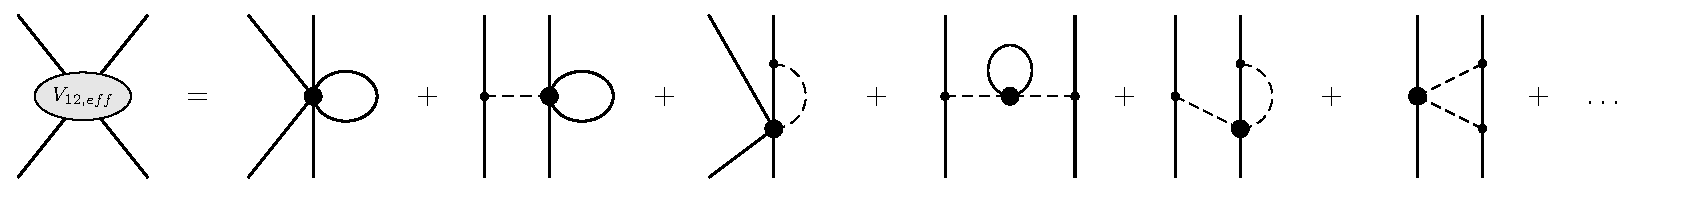
\includegraphics[scale=0.6,page=1]{Figures/InMediumDiagrams2}
\caption{\label{fig:eff-diagram} Diagrammatic representation of $V_{12,\text{eff}}$.}
\end{figure}
 We have made the approximation that the net momentum of the spectator particles is zero with respect to the center of mass frame for the Fermi gas, so that the relative initial state and final state momenta are given by
 \begin{equation}
 \vec{k}=\frac{\vec{k}_1-\vec{k}_2}{2},\qquad \vec{k}'=\frac{\vec{k}'_1-\vec{k}'_2}{2}
 \end{equation}
 
 % What is best way to notate \tau_3(1) type operators?
 The effective interactions for \eqref{eq:V_E} and \eqref{eq:V_D} are given in momentum space by
 \begin{align}
 \veff^E=-&\frac{3c_Em_\pi^3}{2F_\pi^4 \Lambda_\chi}\left(\rhozero-\rhoone\tauplusthree\right)\\
 \begin{split}
 \veff^D=-&\frac{c_Dg_A m_\pi^3}{8 F_\pi^4\Lambda_\chi}\left[\rhozero\taudot \frac{\vec{\sigma}_1\cdot\vec{q}\:\vec{\sigma}_2\cdot\vec{q} }{q^2+m_\pi^2}  - \rhoone \tauplusthree\frac{\vec{\sigma}_1\cdot\vec{q}\:\vec{\sigma}_2\cdot\vec{q} }{q^2+m_\pi^2} \right. \\
&\left. \vphantom{\frac{1}{1}}+ (3-\taudot\sigmadot) \left(\Gamma_{I=0}(k)+\Gamma_{I=0}(k')\right)  -(1+\sigmadot)\tauplusthree \left(\Gamma_{I=1}(k) + \Gamma_{I=1}(k')\right) \right]
 \end{split} 
 \end{align}
Evaluating the isospin  of these vanish for systems built purely of neutrons or protons. The functions $\Gamma_{I=0,1}(k)=\Gamma_{P}(k)\pm\Gamma_{N}(k)$ are momentum dependent analogues of the densities \eqref{eq:densities} which arise from integrating over the spectator momentum,
 \begin{equation}
 \begin{split}
 \Gamma_{N,P}(k)&=\frac{1}{m_\pi^3}\int^{|k_\delta|<k_F^{N,P}}\frac{d^3\vec{k}_\delta}{(2\pi)^3} \frac{(\vec{k}-\vec{k}_\delta)^2}{(\vec{k}-\vec{k}_\delta)^2+m_\pi^2} \\
 &=\frac{\rho_{N,P}}{8m_\pi^3}\left(2\left[2-3\tilde{m}_\pi^2+3\tilde{m}_\pi^3\left(\arctan\frac{1-\tilde{k}}{\tilde{m}_\pi}+\arctan\frac{1+\tilde{k}}{\tilde{m}_\pi}\right)\right]\right. \\
 &\left.\qquad\qquad\qquad\qquad\qquad-\frac{3}{2 \tilde{k}}\tilde{m}_\pi^2\left(\tilde{k}^2-\tilde{m}_\pi^2-1\right)\log\frac{\tilde{m}_\pi^2+(\tilde{k}-1)^2}{\tilde{m}_\pi^2+(\tilde{k}+1)^2}\right)
 \end{split}
 \end{equation}
All variables appear in the dimensionless combinations $\tilde{m}_\pi=m_\pi/k_F^{N,P}$ and $\tilde{k}=k/k_F^{N,P}$. For actual calculations, one can replace $k_F$ with the observable densities using \eqref{eq:kF}.%$k_F^{N,P}=\left(3\pi^2 \rho_{N,P}\right)^{1/3}$.

\begin{align}
 \veff^{c_1}=-&c_1 m_\pi^5\left(\frac{g_A}{F_\pi^2}\right)^2 \left[ \rhozero\vec{\tau}_1\cdot\vec{\tau}_2 \:\frac{\vec{\sigma}_1\cdot\vec{q}\:\vec{\sigma}_2\cdot\vec{q} }{\left(q^2+m_\pi^2\right)^2} \right]
\end{align}
 
\section{The effective potential in coordinate space}

By evaluating the Fourier transforms of the momentum space effective potential, we obtain the potential in coordinate space. Each term in the full potential contains couplings of varying numbers of vector operators operating on spatial and spin quantum numbers. Throughout, we give the potentials by first coupling any coordinate operators with one another (e.g. forming the spherical harmonics $Y_l(\hat{r}_{12})$ and $Y_l(\rotphat)$), then coupling these operators together before finally coupling with the spin operators.

The simplest of the three-body interactions at N$^2$LO is the contact term. Evaluation of the diagram and summation over the core particles gives the two-body effective potential,
\begin{equation}
V_{12,\text{eff}}(\vec{r}_{12})=\frac{c_E m_\pi^6}{2F_\pi^4\Lambda_\chi}\:\frac{3\delta^{(3)}(\vec{r}_{12})}{m_\pi^3}\left[-\rho_{I=0}+ \rho_{I=1}\tauplusthree \right]
\end{equation}
%where the dimensionless isoscalar and isovector spectator nucleon densities are given by,
%\begin{equation}\label{eq:densities}
%\rho_{I=0,1}=\frac{\rho_P\pm\rho_N}{m_\pi^3}
%\end{equation}

The three-body one pion exchange term (the middle diagram in Figure \ref{fig:3NF}) generates a richer effective interaction. The momentum dependence generates both a purely local interaction
\begin{equation}\begin{split}
V^{D}_{12,\text{eff}}(\rot)=&\frac{c_D g_Am_\pi^6}{8 F_\pi^4 \Lambda_\chi}\: \left[\rho_{I=0}\left(\taudot W^{\text{LR}}_{1PE}(\rot)  +3\frac{\delta^{(3)}(\rot)}{m_\pi^3}\right) \right. \\
&-\left. \rho_{I=1} \left(W^{\text{LR}}_{1PE}(\rot)+(1-2\sigmadot/3)\frac{\delta^{(3)}(\rot)}{m_\pi^3}\right) \frac{\tau_3(1)+\tau_3(2)}{2} \right]
\end{split}
\end{equation}
and a nonlocal potential arising from the exchange terms (DELTA FUNCTIONS HAVE DIMENSIONALITY!)
\begin{equation}\begin{split}\label{eq:1PENonlocal}
V^{D}_{12,\text{eff}}(\rot,\rotp)=\frac{-c_D g_A m_\pi^6}{8 F_\pi^4 \Lambda_\chi}\: \left[ \delta^{(3)}(\rot)\left\{\frac{\hat{\rho}_{I=0}(r'_{12})}{2}\left(\taudot W^{\text{LR}}_{1PE}(\rotp)+\frac{3}{4\pi}\yukawadimless{r'_{12}}\right) \right.\right.& \\
\left.\left.+\frac{\hat{\rho}_{I=1}(r'_{12})}{2}\frac{\tau_3(1)+\tau_3(2)}{2} \left( W^{\text{LR}}_{1PE}(\rotp)-\frac{1}{4\pi}\yukawadimless{r'_{12}}\right) \right\} + \rot \leftrightarrow \rotp \vphantom{\left(\yukawa{r}^2\right)} \right]\hspace{-.25cm}&
\end{split}\end{equation}
In order to highlight the physical meaning of these terms, we write a dimensionless version of the long range terms in the two-body one pion exchange potential as
\begin{equation}\begin{split}
W^{\text{LR}}_{1PE}(\vec{r})&=\frac{1}{12 \pi}\frac{e^{-m_\pi r}}{m_\pi r}\left[\left(3\vec{\sigma}_1\cdot\hat{r}\:\vec{\sigma}_2\cdot\hat{r}-\sigmadot\right)\left(1+\frac{3}{m_\pi r}+\frac{3}{(m_\pi r)^2}\right)+\sigmadot\right] \\
&=\frac{1}{4 \pi}\frac{e^{-m_\pi r}}{m_\pi r}\left[\sqrt{\frac{8\pi}{15}}Y_2(\hat{r})\cdot\sigmatwo\left(1+\frac{3}{m_\pi r}+\frac{3}{(m_\pi r)^2}\right)+\frac{\sigmadot}{3}\right]
\end{split}
\end{equation}

The density dependence is now also mixed with spatial dependence, which we define in analogy with \eqref{eq:densities} as 
\begin{equation}\label{eq:hatdensities}
\hat{\rho}_{I=0,1}(r)=%\frac{\rho_P}{m_\pi^3}\:\frac{3 j_1(k^P_F r)}{k_F^P r}\pm\frac{\rho_N}{m_\pi^3}\:\frac{3 j_1(k^N_F r)}{k_F^N r}=
\frac{1}{m_\pi^3}\left[ \left(\frac{3 \rho_P}{\pi}\right)^{2/3} \frac{ j_1( [3\pi^2 \rho_P]^{1/3}  r)}{ r} \pm \left(\frac{3 \rho_N}{\pi}\right)^{2/3} \frac{ j_1( [3\pi^2 \rho_N]^{1/3}  r)}{ r} \right]
\end{equation}

For all pieces of the N$^2$LO 3N interaction besides the purely short range contact $V_E$, nonlocal effective interactions like \eqref{eq:1PENonlocal} are generated from summing over terms which are not diagonal in the spectator particle. Coordinate space potentials are generally nonlocal when there is a momentum dependence of the interaction. In this case, the $\Gamma$ terms with complicated momentum dependence in Section \ref{sec:momentum} are the source.

From the 2PE term, a large number of unique terms are generated for the effective interaction. The $V_1$ piece again produces both a local part 
\begin{multline}
V^{1}_{12,\text{eff}}(\rot)=-\frac{c_1 m_\pi^6}{8\pi}\left(\frac{g_A}{F_\pi^2}\right)^2 \rho_{I=0}\taudot\:\\
 \times\left(\sqrt{\frac{8\pi}{15}}Y_2(\hat{r})\cdot\sigmatwo \w{2}{2}{2}{m_\pi r} +\frac{\sigmadot}{3}  \w{2}{2}{0}{m_\pi r} \right)
\end{multline}
and a nonlocal part 

\begin{multline}
V^{1}_{12,\text{eff}}(\rot,\rotp)=-\frac{c_1 m_\pi^9}{48\pi} \left(\frac{g_A}{F_\pi^2}\right)^2 
\left\{ \vphantom{\frac{1}{3}} \right. \\
\left[ \taudot \: \rhohat{0}{|\rot-\rotp|} + \tau_3(1) \rhohat{1}{|\rot-\rotp|} \right] \w{1}{1}{1}{m_\pi r_{12}} \w{1}{1}{1}{m_\pi | \rot-\rotp | }\\
\times \left( \sigmatwo \cdot [ Y_1 (\hat{r}_{12}) \otimes Y_1 \left(\frac{\rot-\rotp}{|\rot-\rotp|}\right) ]_2
 +\frac{1}{2}(\sigmacross)\cdot (Y_1 (\hat{r}_{12}) \times Y_1 \left(\frac{\rot-\rotp}{|\rot-\rotp|}\right) ) \right. \\
\left.+\frac{\sigmadot}{3} Y_1 (\hat{r}_{12}) \cdot Y_1 \left(\frac{\rot-\rotp}{|\rot-\rotp|}\right)
+\rot\leftrightarrow\rotp\right) \\
+\left[3\rhohat{0}{|\rot-\rotp|}-\tau_3(1)\rhohat{1}{|\rot-\rotp|}\right] \w{1}{1}{1}{m_\pi r_{12}} \w{1}{1}{1}{m_\pi \rotpr} \\
\times\left.\left(i\vec{\sigma}_1 \cdot (Y_1 (\hat{r}_{12}) \times Y_1(\rotphat)) + Y_1 (\hat{r}_{12}) \cdot Y_1(\rotphat) \fracphantom \right)
\right\}
\end{multline}

The $V_4$ term generates only a nonlocal term because the terms diagonal in the spectator particle all sum to zero. The nonlocal terms are

\begin{multline}
V^{4}_{12,\text{eff}}(\rot,\rotp) = \frac{c_4}{4}\frac{g_A^2}{F_\pi^2}\frac{m_\pi^9}{16\pi^2}\left\{ \fracphantom \right. \\
\rhohat{0}{|\rot-\rotp|}\taudot\left( -\frac{4}{3}\sqrt{\frac{8\pi}{15}}\sigmatwo\cdot Y_2(\rotphat)\w{2}{1}{2}{m_\pi \rotpr}\w{2}{1}{0}{m_\pi |r_{12}- \rotpr|} \right. \\
+\frac{2}{9}\sigmadot\; \w{2}{1}{0}{m_\pi \rotpr}\w{2}{1}{0}{m_\pi |r_{12}- \rotpr|} \\
+\sqrt{\frac{7}{12}}\frac{8\pi}{15}\sigmatwo\cdot \left[ Y_2(\rotphat)\otimes Y_2 \left(\frac{\rot-\rotp}{|\rot-\rotp|}\right) \right]_2 \w{2}{1}{2}{m_\pi \rotpr}\w{2}{1}{2}{m_\pi |r_{12}- \rotpr|} \\
-\frac{1}{3}\frac{8\pi}{15}\sigmadot \; Y_2(\rotphat)\cdot Y_2\left(\frac{\rot-\rotp}{|\rot-\rotp|}\right) \w{2}{1}{2}{m_\pi \rotpr}\w{2}{1}{2}{m_\pi |r_{12}- \rotpr|} \\
-\frac{1}{3}\sqrt{\frac{8\pi}{15}}\sigmatwo\cdot Y_2\left(\frac{\rot-\rotp}{|\rot-\rotp|}\right)\w{2}{1}{0}{m_\pi \rotpr}\w{2}{1}{2}{m_\pi |r_{12}- \rotpr|} \\
\left.-\; \rot \leftrightarrow \rotp \fracphantom\right) \\
\rhohat{0}{|\rot-\rotp|}\taudot \left( -\sqrt{\frac{5}{2}} \frac{8\pi}{15} \frac{\sigmaplus}{2}\cdot\left[Y_2(\hat{r}_{12})\otimes Y_2(\rotphat)\right]_1 \w{2}{1}{2}{m_\pi r_{12}} \w{2}{1}{2}{m_\pi \rotpr}\right. \\
-\frac{\sqrt{21}}{3}\frac{8\pi}{15}\sigmatwo \cdot \left[Y_2(\hat{r}_{12})\otimes Y_2(\rotphat)\right]_2 \w{2}{1}{2}{m_\pi r_{12}} \w{2}{1}{2}{m_\pi \rotpr} \\
-\frac{1}{3}\frac{8\pi}{15}\sigmadot\; Y_2(\hat{r}_{12}) \cdot Y_2(\rotphat)\w{2}{1}{2}{m_\pi r_{12}} \w{2}{1}{2}{m_\pi \rotpr} \\
+\frac{2}{9}\sigmadot \;\w{2}{1}{0}{m_\pi r_{12}} \w{2}{1}{0}{m_\pi \rotpr} \\
+\frac{1}{3}\sqrt{\frac{8\pi}{15}} \sigmatwo \cdot Y_2(\hat{r}_{12}) \w{2}{1}{2}{m_\pi r_{12}} \w{2}{1}{0}{m_\pi \rotpr} \\
+\frac{1}{3}\sqrt{\frac{8\pi}{15}} \sigmatwo \cdot Y_2(\rotphat) \w{2}{1}{0}{m_\pi r_{12}} \w{2}{1}{2}{m_\pi \rotpr} \left.\fracphantom\right)\\
+\rhohat{1}{|\rot-\rotp|}\tauplusthree \left(\frac{4}{3} \sqrt{\frac{8\pi}{15}} \sigmatwo \cdot Y_2(\rotpr) \w{2}{1}{0}{m_\pi \rotphat} \w{2}{1}{2}{m_\pi |r_{12}- \rotpr|} \right. \\
-\frac{2}{9} \sigmadot \w{2}{1}{0}{m_\pi \rotphat} \w{2}{1}{0}{m_\pi |r_{12}- \rotpr|} \\
-\frac{\sqrt{7}}{12}\frac{8\pi}{15} \sigmatwo \cdot \left[ Y_2(\rotphat)\otimes Y_2 \left(\frac{\rot-\rotp}{|\rot-\rotp|}\right) \right]_2 \w{2}{1}{2}{m_\pi \rotpr}\w{2}{1}{2}{m_\pi |r_{12}- \rotpr|} \\
+\frac{1}{3}\frac{8\pi}{15} \sigmadot \; Y_2(\rotphat)\cdot Y_2\left(\frac{\rot-\rotp}{|\rot-\rotp|}\right) \w{2}{1}{2}{m_\pi \rotpr}\w{2}{1}{2}{m_\pi |r_{12}- \rotpr|} \\
+\frac{1}{3}\sqrt{\frac{8\pi}{15}}\sigmatwo\cdot Y_2\left(\frac{\rot-\rotp}{|\rot-\rotp|}\right)\w{2}{1}{0}{m_\pi \rotpr}\w{2}{1}{2}{m_\pi |r_{12}- \rotpr|}\left.-\; \rot \leftrightarrow \rotp \fracphantom\right) 
\displaybreak[4]\\
%
%
\rhohat{1}{|\rot-\rotp|}\tauplusthree \left( \frac{\sqrt{21}}{3}\frac{8\pi}{15}\sigmatwo \cdot \left[Y_2(\hat{r}_{12})\otimes Y_2(\rotphat)\right]_2 \w{2}{1}{2}{m_\pi r_{12}} \w{2}{1}{2}{m_\pi \rotpr} \right. \\
+\frac{1}{3}\frac{8\pi}{15}\sigmadot\; Y_2(\hat{r}_{12}) \cdot Y_2(\rotphat)\w{2}{1}{2}{m_\pi r_{12}} \w{2}{1}{2}{m_\pi \rotpr} \\
-\frac{2}{9}\sigmadot \;\w{2}{1}{0}{m_\pi r_{12}} \w{2}{1}{0}{m_\pi \rotpr} \\
-\frac{1}{3}\sqrt{\frac{8\pi}{15}} \sigmatwo \cdot Y_2(\hat{r}_{12}) \w{2}{1}{2}{m_\pi r_{12}} \w{2}{1}{0}{m_\pi \rotpr} \\
-\frac{1}{3}\sqrt{\frac{8\pi}{15}} \sigmatwo \cdot Y_2(\rotphat) \w{2}{1}{0}{m_\pi r_{12}} \w{2}{1}{2}{m_\pi \rotpr} \left.\fracphantom\right)\\
\rhohat{1}{|\rot-\rotp|}\tauminusthree \left( \frac{\sqrt{5}}{2} \frac{8\pi}{15} \sigmaone \cdot \left[ Y_2(\hat{r}_{12}) \otimes Y_2(\rotphat)\right]_1 \w{2}{1}{2}{m_\pi r_{12}} \w{2}{1}{2}{m_\pi \rotpr} 
\right.
\end{multline}


%\begin{multline}
%V^{1}_{12,\text{eff}}(\rot,\rotp)=c_1 m_\pi^6\left(\frac{g_A}{F_\pi^2}\right)^2 \left[\vphantom{\frac{1}{3}}\right. \\
%  \frac{4\pi}{3}\left(1+\frac{1}{m_\pi r_{12}}\right)\yukawadimless{r_{12}}\left(1+\frac{1}{m_\pi |r_{12}-r_{12}'|}\right)\yukawadimless{|r_{12}-r'_{12}|} \\
%   \times\left\{\left[\vphantom{x^{i}}
%   \hat{\rho}_{I=0}(\rot-\rotp) \taudot+\hat{\rho}_{I=1}(\rot-\rotp)\tau_3(1)\right]
%   \left(\vec{\sigma}_1\cdot Y_{1}(\hat{r}'_{12})\vec{\sigma}_2\cdot Y_{1}(\hat{r_{12}-r'_{12}})+\rot\leftrightarrow\rotp\right) \right.\\
%\left.+i\taucrossthree\hat{\rho}_{I=1}(\rot-\rotp)\left(\vec{\sigma}_1\cdot Y_{1}(\hat{r}'_{12})\vec{\sigma}_2\cdot Y_{1}(\hat{r_{12}-r'_{12}})-\rot\leftrightarrow\rotp\right)\right\} \\
%+ \frac{4\pi}{3}\left(1+\frac{1}{m_\pi r_{12}}\right)\yukawadimless{r_{12}}\left(1+\frac{1}{m_\pi r'_{12}}\right)\yukawadimless{r'_{12}} \\
%\times \left[3\vphantom{x^{i^i}}\hat{\rho}_{I=0}(\rot-\rotp)-\hat{\rho}_{I=1}(\rot-\rotp)\tau_3(1)\right]\vec{\sigma}_1\cdot Y_{1}(\hat{r}_{12})\vec{\sigma}_1\cdot Y_{1}(\hat{r}'_{12})\left.\vphantom{\frac{1}{3}}\right].
%\end{multline}


\section{A first order local expansion}

Although nonlocality is a common feature of nuclear potentials \cite{PhysRevC.53.R1483}, working with local potentials is typically simpler and less computationally expensive. In light of this, we develop here a local approximation to the full density-dependent effective interaction.

The nonlocal parts can be systematically Taylor expanded in the coordinate $m_\pi(\vec{r}-\vec{r}\:')/2$ to give a series of purely local terms. To estimate the size of this expansion parameter, consider the naive model of an isospin symmetric nucleus with a spherical potential well. The size of the expansion parameter is bounded by the radius of the nucleus, so that 
\begin{equation}
m_\pi(\vec{r}-\vec{r}\:')/2 \lesssim 
\end{equation}

\appendix

\section{\label{app:wNotation}Fourier integrals}

Similar to \cite{PhysRevC.85.024003}, we introduce the following notation for the dimensionless radial functions $\w{\alpha}{\beta}{\ell}{ m r }$, defined by

\begin{align}
i^\ell \, Y_\ell(\hat{r}) \, \w{\alpha}{\beta}{\ell}{ m r}  &= \frac{4 \pi}{m^{3+\alpha-2\beta} }  \int \frac{d^3 q}{(2\pi)^3} \frac{q^\alpha}{(q^2+m^2)^\beta} Y_\ell(\hat{q}) \, e^{i \mathbf{q} \cdot \mathbf{r}  },
\end{align}
which implies that
\begin{align}\label{eq:wDef}
\w{\alpha}{\beta}{\ell}{z} =  \frac{2}{\pi} \int dk \, k^2 \, \frac{k^\alpha}{(1+k^2)^\beta} j_\ell(k z)
\end{align}
with $\vec{z} \equiv m \vec{r}$ and $k$ both dimensionless. Below, we tabulate this integral for selected values of $\alpha, \beta, \ell$. The first function we recover, for the case of $(\alpha, \beta, \ell ) = (0,1,0)$, is nothing but a Yukawa potential. 

To further demonstrate the use of this integral, we now derive the familiar tensor force resulting from one pion exchange. This amplitude is related to the integral
\begin{equation} 
V_\pi( \mathbf{r}) =  -\frac{g_A^2 }{4 F_\pi^2} \:\taudot \int \frac{d^3 q } {(2 \pi)^3 } \frac{(\sigma^{(1)} \cdot \mathbf{q} ) (\sigma^{(2)} \cdot \mathbf{q} ) } {q^2+m_\pi^2} e^{i \mathbf{q} \cdot \mathbf{r} }. 
\end{equation}
We can rewrite the numerator in the integral as
\begin{equation} (\sigma^{(1)} \cdot \mathbf{q}) ( \sigma^{(2)} \cdot \mathbf{q} )= q^2 \left(\sqrt{\frac{8\pi}{15}} [\sigma^{(1)} \otimes \sigma^{(2)}]_2 \cdot Y_2(\hat{q}) + \tfrac{1}{3} \sigma^{(1)} \cdot \sigma^{(2)}  Y_0(\hat{q}) \right),\end{equation}
which then gives
\begin{equation} 
V_\pi( \mathbf{r}) = - \frac{g_A^2 }{4 F_\pi^2} \taudot \left(\frac{m_\pi^3}{4 \pi}\right) \left\{ - \sqrt{\frac{8\pi}{15}} [\sigma_1 \otimes \sigma_2]_2 \cdot Y_2(\hat{r}) \w{2}{1}{2}{m_\pi r} + \frac{1}{3} \sigma_1 \cdot \sigma_2 \w{2}{1}{0}{m_\pi r } \right\},  \end{equation}
or, plugging in explicit values for the $w$'s from Table \ref{table:wTable} and recalling that the tensor operator $S_{12}$ is conventionally defined
\begin{equation}
S_{12} \equiv   3\vec{\sigma}_1\cdot \hat{r}\vec{\sigma}_2\cdot \hat{r} -\sigmadot = 3\:\sqrt{\frac{8\pi}{15}} \:[\sigma_1 \otimes \sigma_2]_2 \cdot Y_2(\hat{r}) , 
\end{equation}
we have
\begin{equation} V_\pi( \mathbf{r})= \frac{g_A^2 }{4 F_\pi^2}  \left(\frac{m_\pi^3}{12 \pi}\right) \left\{ \frac{e^{-m_\pi r}}{m_\pi r} \left[ S_{12}\left(1+\frac{3}{m_\pi r}+ \frac{3}{m_\pi^2 r^2} \right) +  \sigma_1 \cdot \sigma_2 \right] - 4\pi  \sigma_1 \cdot \sigma_2 \delta^3(m_\pi \mathbf{r}) \right\}, 
\end{equation}
which is the familiar result.
\begin{table}
\begin{center}
\begin{tabular}{| c c c | c |}
\hline
$\alpha$ & $\beta$ & $\ell$ & $ \w{\alpha}{\beta}{\ell}{z}$ \\
\hline
0 & 0 & 0 & $ 4\pi \delta^{(3)}(\vec{z}) $ \\
0 & 1 & 0 & $ \frac{\displaystyle e^{-z}}{\displaystyle z} $ \\
2 & 1 & 0 & $ -\frac{\displaystyle e^{-z}}{\displaystyle z} + 4\pi \delta^{(3)}(\vec{z}) $ \\
1 & 1 & 1 &  $\frac{\displaystyle e^{-z}}{\displaystyle z} (1 + \tfrac{1}{z})  $ \\
2 & 1 & 2 & $ \frac{\displaystyle e^{-z}}{\displaystyle z} (1+ \tfrac{3}{z} + \tfrac{3}{z^2} )$ \\
2 & 2 & 0 & $ \frac{\displaystyle e^{-z}}{\displaystyle z} (-\tfrac{z}{2} + 1 ) $ \\
2 & 2 & 2 & $  \frac{\displaystyle e^{-z}}{\displaystyle z} (\tfrac{z}{2} + \tfrac{1}{2} ) $ \\
4 & 2 & 0 & $  \frac{\displaystyle e^{-z}}{\displaystyle z} (\tfrac{z}{2} - 2 ) + 4 \pi \delta^3( \vec{z} )  $ \\
4 & 2 & 2 & $  \frac{\displaystyle e^{-z}}{\displaystyle z} ( - \tfrac{z}{2} + \tfrac{1}{2} + \tfrac{3}{z} + \tfrac{3}{z^2} ) $ \\
\hline
\end{tabular}
\end{center}
\caption{\label{table:wTable} Table of selected values for $\w{\alpha}{\beta}{\ell}{z}$ found by integrating equation \eqref{eq:wDef}.}
\end{table}


\bibliography{References}
\end{document}
%
% ****** End of file apssamp.tex ******
